\chapter{Thảo luận\label{chapter:discussion}}

\section{Tóm tắt phát hiện}
Câu trả lời cho RQ1 chia tại bão hoà. Dưới đó các biến thể khớp nhau đến $\PFiftyRange\,\mu$s ở
trung vị, và đuôi xa phân giải nghiêng về \FarTailLower{}. Vòng khứ hồi đầu-cuối chỉ là
$\BudgetCoreShareMax\%$ công việc ngôn ngữ, nên nó không thể giới hạn một hiệu ứng ngôn ngữ.
Cùng thao tác đo riêng nhanh hơn $\BudgetCoreRatio\times$ ở \BudgetCoreFaster{}. Qua bão hoà
chúng phân kỳ theo cả hai chiều. Các nhánh Rust giữ tốc độ đưa vào đến $\TrackingLoadRust$~kops/s
đối với $\TrackingLoadCpp$. Tại $\OverloadLoad$~kops/s \OverloadSustainedFaster{} duy trì
$\OverloadThrRatio\times$ thông lượng của \OverloadSustainedSlower{}.
RQ2 là kết quả đã chốt và không phụ thuộc máy chủ. Cả bảy lớp trong bảo đảm đều là lỗi biên dịch
trong Rust an toàn. Cả bảy lớp biên đều biên dịch và hành xử sai ở cả hai ngôn ngữ. RQ3 là một
phạt bộ nhớ $\RssLangDiffLo$--$\RssLangDiffHi$~MiB tái hiện dưới cả hai bộ cấp phát và trên cả
ba máy, với CPU đảo dấu qua hai chế độ tải. RQ4 là một đường nối nhỏ mà thuế mỗi lần gọi được
giới hạn ở $\FfiOpBoundPct\%$ của cuộc gọi đó. Chi phí thực là thiết kế API và đường cong học
tập.

\section{Thảo luận các câu hỏi nghiên cứu}\label{sec:rqdiscussion}
Việc một triển khai nên làm gì với RQ1 phụ thuộc nơi nó kỳ vọng ngồi, không phụ thuộc một xếp
hạng đơn. Một dịch vụ được định cỡ để chạy dưới điểm gối của mỗi nhánh nên chọn nhánh giữ tốc độ
đưa vào xa hơn. Một dịch vụ mà một cơn bão báo hiệu sẽ đẩy qua mỗi điểm gối nên chọn nhánh vẫn hoàn
thành nhiều việc hơn sau đó. Hai ưa thích đó hướng tới hai ngôn ngữ đối lập. Chỉ cái thứ hai
được thử. Cái thứ nhất là mô tả, vì lý do Mục~\ref{sec:overload} đưa. Một phép so sánh dừng ở
tải mà dịch vụ vẫn đáp sẽ đọc chiều ngược với cùng bộ máy.

Công trình trước gần nhất đo đại lượng này cho các thủ tục mặt điều khiển 5G. Nó tìm cùng hình
dạng và truy nó về \texttt{async}/\texttt{await} không ngăn xếp~\cite{arvidsson2025async}. Quy
kết đó được chấp nhận ở đây. Hình dạng xuất hiện mà không có thời gian chạy bất đồng bộ ở phía
nào và mô hình tương tranh được giữ cố định. Một thời gian chạy không thể là nơi duy nhất một
hiệu ứng như vậy phát sinh. Dự đoán đăng ký trước cũng nêu nơi nhìn trước, kiểm biên và kiểm
overflow~\cite{zhang2022runtime,harris2023morello}. Phần đó của nó sai. Khoảng cách trung vị
khớp với bằng chứng rằng các kiểm an toàn của Rust phần lớn được CPU hiện đại ra-khỏi-thứ-tự
hấp thụ~\cite{balasubramanian2017rust,emmerich2019drivers}. Nó cũng yếu hơn vẻ ngoài. Thao tác
lõi là $\BudgetCoreShareMax\%$ những gì quét đo.

Về an toàn, một số lỗi không thể chạm một nhị phân chút nào. Bảy lớp Rust không ngăn là một phần
của câu trả lời, không phải một cảnh báo thêm sau. Một trình biên dịch từ chối xây một chương
trình loại lỗi khỏi mỗi lần thực thi. Một bộ dò lỗi chỉ loại nó khỏi những lần chạy mà một kiểm
thử bộ dò lỗi tình cờ đi. Cái tuyệt đối ở đó là phủ thực thi, không phải bề rộng của danh mục.
Hình~\ref{fig:boundary} nêu cơ chế mỗi bên của đường đó. Rust lý luận về aliasing chứ không về
thứ tự chiếm. Một guard \texttt{Mutex} mà bộ kiểm mượn theo dõi vòng đời hoàn hảo không nói gì
về việc hai luồng lấy khoá theo thứ tự tương thích. Phát hiện khoá chết tĩnh cho Rust là một bài
toán nghiên cứu đang mở~\cite{zhang2026deadlock}. Lost update thoát ThreadSanitizer vì cùng lý
do nó thoát bộ kiểm mượn. Nơi mỗi truy cập được đồng bộ đúng, không có truy cập không đồng bộ để
tìm. Trong một nghiên cứu hiện trường $105$ lỗi tương tranh thực, khoảng một phần ba các trường
hợp không phải khoá chết vi phạm thứ tự lập trình viên định chứ không phải việc
khoá~\cite{lu2008mistakes}. Áp dụng Rust loại một hạng lỗi tương tranh và để nguyên hạng thất
bại trong im lặng. Một kế hoạch di trú đọc ``an toàn bộ nhớ'' như ``an toàn tương tranh'' sẽ
tính sai ngân sách rà soát. Lỗi an toàn bộ nhớ trong Rust dính \texttt{unsafe} trong mọi mục
Common Vulnerabilities and Exposures (CVE) đã công bố trừ một lỗi trình biên
dịch~\cite{xu2021rustcve}, đó là lý do giữ lõi không \texttt{unsafe} quan trọng, và lý do
mã \texttt{unsafe} lan qua phụ thuộc là mối quan tâm rà soát~\cite{evans2020rust}.

\begin{figure}[ht]
\centering
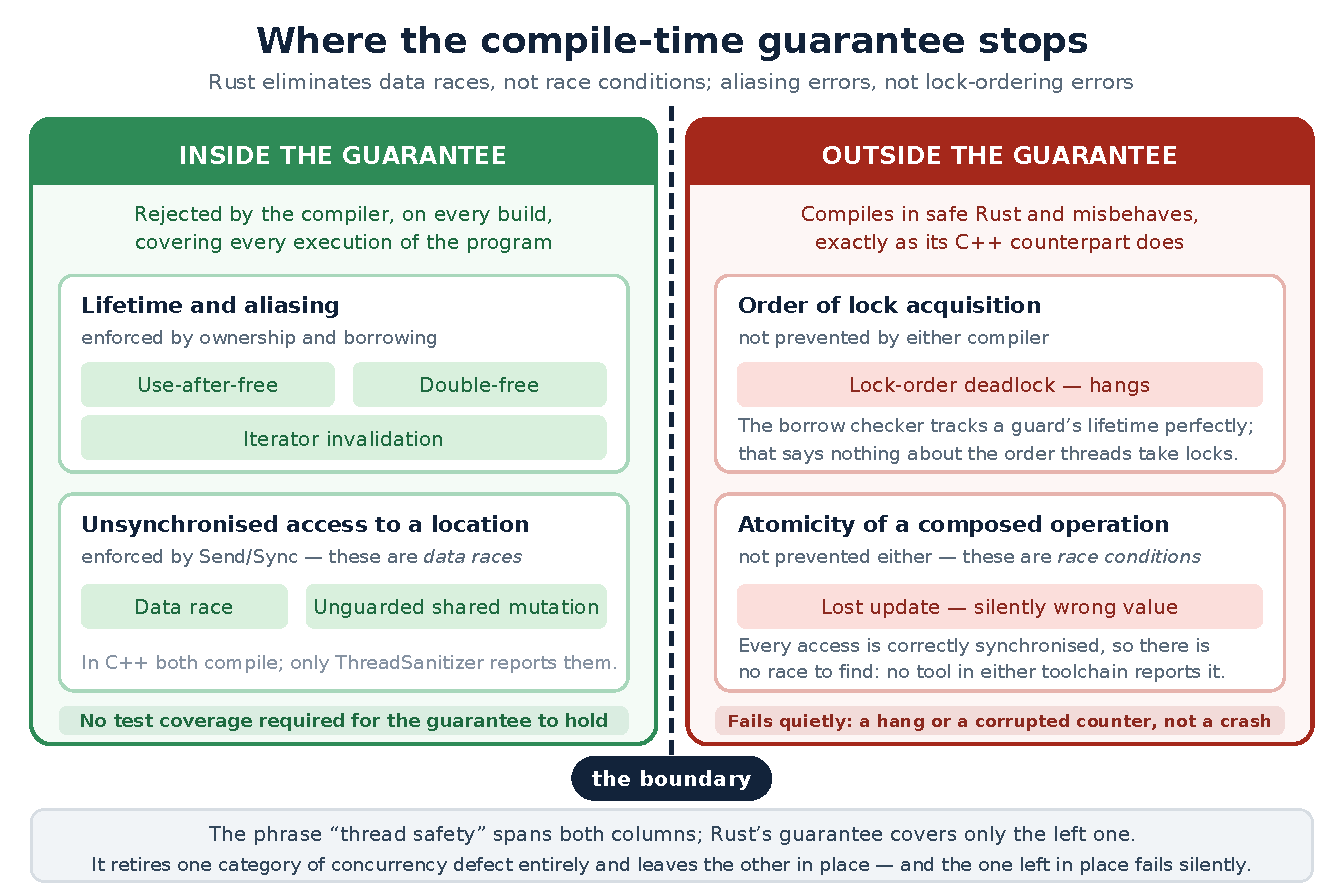
\includegraphics[width=0.78\linewidth]{diagrams/pdf/17_guarantee_boundary.pdf}
\caption[Nơi bảo đảm lúc biên dịch của Rust dừng]{Nơi bảo đảm lúc biên dịch của Rust dừng, các
lớp nhóm theo cơ chế từ chối chúng.\label{fig:boundary}}
\end{figure}

Một trường hợp vượt quá các chương trình được tiêm. Một lỗ đặc tả cho phép một thao tác được gửi
ngoài cửa sổ chạy của dịch vụ. Nó sống sót mỗi kiểm thử, mỗi vector tương đương và cả ba bộ dò
lỗi vì không gì từng gọi đường đó. Cái biến hành vi không định nghĩa thành một thất bại chẩn
đoán được ở phía Rust là một kiểm biên thông thường, không phải một chứng minh. Thuộc tính đáng
ngân sách là ``được kiểm mặc định'', không phải ``bị loại lúc biên dịch''. Nguyên nhân gốc thuộc
về phương pháp. Một cấm nêu ra mà không có cơ chế phía sau để mỗi bản thất bại theo thành ngữ
của riêng nó.

RQ3 tách theo tài nguyên và các tách không chỉ cùng chiều. Phạt bộ nhớ tái hiện dưới cả hai bộ
cấp phát và trên một máy thứ hai với trình biên dịch khác. Tập trú đỉnh là cực đại cấp lần chạy,
nên độ dao động phá một p99 không chạm nó. Đo so với hiệu ứng của chính bộ cấp phát, hai cái
cùng bậc trên cả hai máy vật lý. Trên máy ảo, của bộ cấp phát lớn hơn một bậc. Hiệu ứng ngôn
ngữ đi được. Tỉ số thì không. Máy yên cũng định vị chi phí ngoài bộ cấp phát, bằng sổ sách của
chính bộ cấp phát. Một nghiên cứu gần báo dấu ngược, Rust thấp nhất và khoảng cách rộng khi
tương tranh tăng~\cite{karlback2021ran}. Hai phát hiện đó khớp nhau khi các nhánh được đọc như
hai thời gian chạy tương tranh. C++ của họ chạy trên Boost.Fibers, cấp một ngăn mỗi fiber. Rust
của họ chạy trên Tokio, nơi một task là một future nhỏ cấp trên heap. Họ đo chi phí mỗi ngữ cảnh
của hai thời gian chạy tương tranh. Hai nghiên cứu nữa khớp chiều tìm thấy ở
đây~\cite{olsson2023ranmgmt,sundvisson2026drivers}. Về CPU dấu phụ thuộc tải. Một số đơn cho
``chi phí CPU của mô hình an toàn Rust'' sẽ trung bình hai chế độ đi ngược chiều.

RQ4 ra rẻ ở máy và đắt ở người. Một máy chủ C++ có thể gọi một lõi Rust không đổi qua một đường
nối C-ABI mỏng mà chi phí trên một cuộc gọi báo hiệu thực được giới hạn ở $\FfiOpBoundPct\%$ của
cuộc gọi đó. Chi phí chiếm ưu thế là con người~\cite{fulton2021adopting,crichton2024learning}. Nhốt
\texttt{unsafe} vào đường nối giới hạn những gì phải rà soát, không phải những gì có thể bị làm
hỏng. Máy chủ và thành phần chia một không gian địa
chỉ~\cite{rivera2021galeed,kirth2022pkrusafe}. Các trục build và dấu chân chỉ cùng chiều với
đường nối. Một nhà cung cấp lo một trong hai nên kiểm ngân sách phụ thuộc trước khi đổ lỗi trình
biên dịch. Trục duy nhất C++ dẫn thẳng là vòng sửa-biên dịch cho các thay đổi nằm trong một đơn
vị dịch. Con số kích thước nhị phân $\FootShippedRatio\times$ so hai chính sách liên kết, và thứ
tự đảo khi chính sách được giữ cố định.

\section{Xem lại các giả thuyết}\label{sec:hypotheses}
Mục~\ref{sec:rqs} cam kết ba giả thuyết trước mọi phép đo. Nêu cách xử chúng là điều tách một
phép thử khỏi một mô tả.

\begin{description}
  \item[H1] Mệnh đề trung vị giữ theo nghĩa thực tiễn. Kiểm định ghép cặp phân giải
        $\PFiftyDiffAbsMax\,\mu$s, quá nhỏ để giới hạn một hiệu ứng ngôn ngữ. Mệnh đề đuôi xa
        không giữ, và quá tải, điều mà cách diễn đạt không bao giờ nêu tên, là nơi các ngôn ngữ
        thực sự tách. Chiến dịch được báo cáo nay phân giải đuôi đó, nghiêng về Rust, và một máy
        vật lý thứ hai đồng ý về chiều. H1 đúng về nơi một khác biệt dưới bão hoà sẽ hiện và sai
        rằng đó là nơi duy nhất. Nó cũng không được đặt tốt. ``Tương đương hiệu năng'' đọc như
        một đại lượng và nêu ít nhất ba: vòng khứ hồi giao dưới bão hoà, mã các trình biên dịch
        phát, và việc bền dưới quá tải. Ba cái đó không đi cùng nhau.
  \item[H2] Với bảy lớp được tiêm cùng loại, nó giữ không ngoại lệ. Nó thất bại ở cách đọc lỏng
        hơn mà cách diễn đạt mời. Nó được chấp nhận cho an toàn bộ nhớ và không tranh chấp dữ
        liệu, bị bác cho tính đúng đắn tương tranh nói chung, và nó là tuyên bố chỉ về Rust
        \emph{an toàn}. Trường hợp đường nối cho thấy cùng lớp trở lại bên trong
        \texttt{unsafe}.
  \item[H3] Mọi thuế mỗi lần gọi được giới hạn ở $\FfiOpBoundPct\%$ của cuộc gọi báo hiệu đó, đó
        là chỗ dựa từ một giới hạn trên một chi phí mà phép đo có thể đã bỏ sót, không từ thất
        bại phát hiện một chi phí. Tuyên bố kèm theo, rằng chi phí thực là thiết kế và đào tạo,
        được chống đỡ về cấu trúc chứ không về thống kê.
\end{description}

\section{Hướng dẫn kỹ thuật cho áp dụng tăng dần}\label{sec:guidelines}
Các hướng dẫn là dạng thực tiễn của các phát hiện, và mỗi cái mang giới hạn của phát hiện đứng
sau. Chọn thành phần đầu vì giao diện hẹp, không vì kích thước. Thiết kế lại một giao diện giàu
là rủi ro lịch. Bản thân biên không phải. Giữ ABI C trong crate riêng và lõi không
\texttt{unsafe}. Điều đó giữ mã \texttt{unsafe} khỏi các chuỗi phụ thuộc mà nó nếu không lan
qua~\cite{evans2020rust}. Để ngân sách rà soát tương tranh ở chỗ cũ. Ưa một cấu trúc không chia
sẻ ở ngôn ngữ nào. Kết quả tương tranh mạnh nhất ở đây thuộc về thiết kế chứ không thuộc trình
biên dịch nào. Lập kế hoạch đường cong học tập như một chi phí đào tạo và đo nó. Đo thành phần
cũng như vòng khứ hồi. Quét qua điểm dịch vụ ngừng chịu được. Đó là hướng dẫn nghiên cứu này
muốn đã theo từ đầu nhất.

\section[Nơi nghiên cứu này đứng]{Nơi nghiên cứu này đứng, và những gì nó không chống đỡ được}\label{sec:standing}
Các nghiên cứu gần nhất với nghiên cứu này là năm luận văn do nhà cung cấp lưu trữ của
Mục~\ref{sec:gap}. Phán quyết của chúng mâu thuẫn nhau theo mỗi chiều. Bài báo dấu ngược trên
bộ nhớ đỉnh hoà với nghiên cứu này khi các nhánh được đọc như hai thời gian chạy tương tranh chứ
không phải hai ngôn ngữ. Ba mối đe dọa vẫn mang sức, và cái đầu là một tác giả viết cả hai bản.
Cùng dạng thất bại đã đảo một phán quyết đã công bố trong ngành này: tương đương sau một rà soát
mã rồi Rust kém hơn $85$--$91\%$ sau tối ưu thêm~\cite{emberg2023asn1}. Bộ tương đương chặn hành
vi chứ không chặn hiệu năng. Dụng cụ đầu-cuối đo thiết kế trung thành và ngôn ngữ hầu như không
đo. Phân kỳ quá tải được tái hiện ở đây với cơ chế được thu hẹp chứ không đóng, và không nghiên
cứu đã bình duyệt nào báo cùng sự đảo.

\section{Suy nghĩ đạo đức và nghề nghiệp}
Nghiên cứu không xử lý dữ liệu cá nhân, thuê bao, hay mật của nhà khai thác. Mọi lưu lượng đều
tổng hợp và phân hệ được mô hình hoá theo mã đang chạy chứ không sao chép từ đó, nên các hiện
vật có thể được phát hành công khai. Trách nhiệm thứ nhất là không tuyên bố quá. Một nhà cung
cấp có thể đọc kết quả RQ2 như giấy phép mô tả một thành phần đã di trú là ``an toàn'', và các
trường hợp biên là lý do cách đọc đó sai. Một mặt điều khiển khoá chết là một sự cố. Một cập
nhật bộ đếm mất trong im lặng có thể làm sai một quyết định di động. Không gì được chứng minh ở
đây ngăn một trong hai. Trách nhiệm thứ hai là bằng chứng đi xa đến đâu. Các số độ trễ đuôi từ
một máy đơn là cơ sở hẹp hơn vẻ ngoài cho một cam kết sản xuất. Đó là lý do chiến dịch máy ảo
trước được báo cáo chứ không bị loại.
